\documentclass{beamer}
\usepackage[utf8]{inputenc}
\usepackage{graphicx}
\usepackage{xspace} % Needed for macro \xspace
\usepackage{fancyvrb} % Needed for the Verbatim environment

% Remove navigation controls
\usenavigationsymbolstemplate{}

% Slide numbering
\setbeamertemplate{footline}[frame number]

% Convienence macro
\newcommand{\atweb}{\textbf{@Web}\xspace}

% Macro for writing an RDF triple
\newcommand{\triple}[1]{$\langle$\texttt{#1}$\rangle$}

\title{An introduction to SHACL}
\subtitle{And its possible uses in the \atweb platform}
\author{
  Leandro Lovisolo \\
  \footnotesize{\href{mailto:leandro.lovisolo@supagro.inra.fr}
                     {leandro.lovisolo@supagro.inra.fr}}
}
\date{October 22, 2015}
\institute{
  INRA SupAgro and INRIA GraphiK \\
  Montpellier, France
}

\begin{document}

\begin{frame}
  \titlepage
\end{frame}

\begin{frame}
  \frametitle{Outline of the presentation}

  \begin{itemize}
    \item Introduction to SHACL
    \item Supported constraints (with examples)
    \item Operations supported by a SHACL engine
    \item An integrity constraint implemented as a SHACL shape
    \item Comparision between SHACL, Shape Expressions and raw SPARQL
  \end{itemize}
\end{frame}

\begin{frame}
  \frametitle{Introduction to SHACL}

  \pause

  \begin{itemize}
    \item SHACL is a language for describing constraints in RDF graphs.

    \pause

    \item Constraints are grouped into \textit{shapes} that apply to nodes in a
      \textit{data graph}.

    \pause

    \item Shapes are described in RDF and stored in a \textit{shapes graph}.

    \pause

    \item The simplest interface to a SHACL processor has two inputs:

    \pause

    \begin{itemize}
      \item A data graph containing the data to be validated

      \pause

      \item A shapes graph containing shape definitions and other information
        that can be used e.g. to determine which nodes in the data graph should
        be evaluated against which shapes
    \end{itemize}
  \end{itemize}
\end{frame}

\begin{frame}[fragile]
  \frametitle{A simple shapes graph}

  \begin{columns}[t]
    \column{0.5\textwidth}

    \begin{Verbatim}[fontsize=\footnotesize]
ex:IssueShape
  a sh:Shape ;
  sh:scopeClass ex:Issue;
  sh:property [
    sh:predicate ex:state ;
    sh:allowedValues (ex:unassigned
                      ex:assigned) ;
    sh:minCount 1 ;
    sh:maxCount 1 ;
  ] ;
  sh:property [
    sh:predicate ex:reportedBy ;
    sh:valueShape ex:UserShape ;
    sh:minCount 1 ;
    sh:maxCount 1 ;
  ] .
    \end{Verbatim}

    \column{0.5\textwidth}

    \begin{Verbatim}[fontsize=\footnotesize]
ex:UserShape
  a sh:Shape ;
  sh:property [
    sh:predicate foaf:name ;
    sh:datatype xsd:string ;
    sh:minCount 1 ;
    sh:maxCount 1 ;
  ] ;
  sh:property [
    sh:predicate foaf:mbox ;
    sh:nodeKind sh:IRI ;
    sh:minCount 1 ;
  ] .
    \end{Verbatim}
  \end{columns}
\end{frame}

\begin{frame}[fragile]
  \frametitle{An example of a corresponding valid data graph}

  \begin{columns}[t]
    \column{0.5\textwidth}

    \begin{Verbatim}[fontsize=\footnotesize]
inst:Issue1
  a ex:Issue ;
  ex:state ex:unassigned ;
  ex:reportedBy inst:User2 .

inst:User2
  a foaf:Person ;
  foaf:name "Bob Smith" ;
  foaf:mbox <mailto:bob@example.org> ;
  foaf:mbox <mailto:rs@example.org> .
    \end{Verbatim}

    \column{0.5\textwidth}

    \begin{Verbatim}[fontsize=\footnotesize]
inst:Issue3
  a ex:Issue ;
  ex:state ex:unsinged ;
  ex:reportedBy inst:User4 .

inst:User4
  a foaf:Person ;
  foaf:name "Bob Smith",
            "Robert Smith" ;
  foaf:mbox <mailto:bob@example.org> ;
  foaf:mbox <mailto:rs@example.org> .
    \end{Verbatim}
  \end{columns}
\end{frame}

\begin{frame}
  \frametitle{Shapes}
  \framesubtitle{Validation process (I)}

  \begin{itemize}
    \item Shapes are instances of the class \texttt{sh:Shape}.

    \pause

    \item A \textit{shape} is a group of constraints that can be validated
      against nodes.

    \pause

    \item If a node is validated against a constraint then it's called the \textit{focus node}.

    \pause

    \item Shapes may have \textit{scopes} that instruct a SHACL processor on
      how to select the focus nodes (e.g. class-based scopes, individual
      scopes, etc.)

    \pause

    \item Shapes may also have \textit{filter shapes} that narrow down the
      scope (e.g. instances of the class that have a certain number of values
      for a given property.)
  \end{itemize}
\end{frame}

\begin{frame}
  \frametitle{Shapes}
  \framesubtitle{Validation process (II)}

  The following picture illustrates the validation process.

  \vspace{1cm}

  \begin{center}
    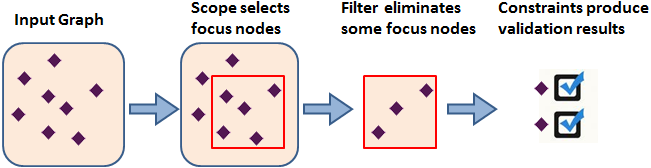
\includegraphics[width=11cm]{shacl-validation-process.png}
  \end{center}
\end{frame}

\begin{frame}[fragile]
  \frametitle{Shape scopes}
  \framesubtitle{Individual scope}

  Individual nodes can point to the shapes they're supposed to be validated
  against using the property \texttt{sh:nodeShape}, e.g.:

  \vspace{1cm}

  \begin{Verbatim}
ex:ExampleShape
  a sh:Shape ;
  sh:constraint [
    ...
  ] .

ex:ExampleInstance
  sh:nodeShape ex:ExampleShape .
  \end{Verbatim}
\end{frame}

\begin{frame}[fragile]
  \frametitle{Shape scopes}
  \framesubtitle{Class-based scope}

  The property \texttt{sh:scopeClass} can be used to link a \texttt{sh:Shape}
  with an \texttt{rdfs:Class} and all its subclasses (by following
  \texttt{rdfs:subClassOf}.)

  \vspace{1cm}

  \begin{Verbatim}[fontsize=\footnotesize]
ex:ExampleClass
  a rdfs:Class .

ex:ExampleShape
  a sh:Shape ;
  sh:scopeClass ex:ExampleClass ;
  sh:constraint [
    ...
  ] .

ex:ExampleInstance
  rdf:type ex:ExampleClass .
  \end{Verbatim}
\end{frame}

\begin{frame}[fragile]
  \frametitle{Shape scopes}
  \framesubtitle{General scopes}

  It's possible to define many kinds of custom scopes. The example below
  selects nodes that have at least one value for property
  \texttt{ex:myProperty}.

  \vspace{1cm}

  \begin{Verbatim}
ex:PropertyScopeExampleShape
  a sh:Shape ;
  sh:scope [
    a sh:PropertyScope ;
    sh:predicate ex:myProperty ;
  ] ;
  sh:constraint [
    ...
  ] .
  \end{Verbatim}
\end{frame}

\begin{frame}[fragile]
  \frametitle{Shape scopes}
  \framesubtitle{Filter shapes}

  Filter shapes are used to apply a shape just to a subset of a scope, e.g.:

  \begin{Verbatim}[fontsize=\footnotesize]
ex:FilteredExampleShape
  a sh:Shape ;
  sh:scopeClass ex:ExampleClass ;
  sh:filterShape [
    sh:property [
      sh:predicate ex:requiredProperty ;
      sh:hasValue ex:requiredValue ;
    ]
  ] ;
  sh:property [
    sh:predicate ex:someProperty ;
    sh:minCount 1 ;
  ] .

ex:FilteredShapeValidExampleInstance
  rdf:type ex:ExampleClass
  ex:someProperty ex:someValue ;
  ex:requiredProperty ex:requiredValue .
  \end{Verbatim}
\end{frame}

\begin{frame}
  \frametitle{Constraints}

  SHACL constraints can be grouped into the following categories:

  \pause

  \begin{itemize}
    \item Property constraints (\texttt{sh:property})

    \pause

    \begin{itemize}
      \item \texttt{sh:hasValue}
      \item \texttt{sh:allowedValues}
      \item \texttt{sh:valueClass}
      \item \texttt{sh:valueShape}
      \item \texttt{sh:minCount}, \texttt{sh:maxCount}
      \item etc.
    \end{itemize}

    \pause

    \item Inverse property constraints (\texttt{sh:inverseProperty})

    \pause

    \item Property pair constraints

    \pause

    \begin{itemize}
      \item \texttt{sh:EqualConstraint}, \texttt{sh:NotEqualConstraint}
      \item \texttt{sh:LessThanConstraint},
        \texttt{sh:LessThanOrEqualConstraint}
      \item etc.
    \end{itemize}

    \pause

    \item Logical constraints

    \pause

    \begin{itemize}
      \item \texttt{sh:NotConstraint}
      \item \texttt{sh:AndConstraint}, \texttt{sh:OrConstraint}
      \item etc.
    \end{itemize}

    \pause

    \item Native constraints (e.g. SPARQL-based)
  \end{itemize}
\end{frame}

\begin{frame}[fragile]
  \frametitle{Constraints}
  \framesubtitle{Property constraints by example (I)}

  Some examples of property constraints:

  \begin{columns}[t]
    \column{0.55\textwidth}

    \begin{Verbatim}[fontsize=\footnotesize]
ex:AllowedValuesExampleShape
  a sh:Shape ;
  sh:property [
    sh:predicate ex:someProperty ;
    sh:allowedValues ( ex:Value1
                       ex:Value2
                       ex:Value3 ) ;
  ] .

ex:AllowedValuesExampleValidRes
  ex:someProperty ex:Value2 .
    \end{Verbatim}

    \column{0.45\textwidth}

    \begin{Verbatim}[fontsize=\footnotesize]
ex:HasValueExampleShape
  a sh:Shape ;
  sh:property [
    sh:predicate ex:property ;
    sh:hasValue ex:Green ;
  ] .

ex:HasValueExampleValidResource
  ex:property ex:Green .
    \end{Verbatim}
  \end{columns}
\end{frame}

\begin{frame}[fragile]
  \frametitle{Constraints}
  \framesubtitle{Property constraints by example (II)}

  \begin{columns}[t]
    \column{0.5\textwidth}

    \begin{Verbatim}[fontsize=\footnotesize]
ex:ValueClassExampleShape
  a sh:Shape ;
  sh:property [
    sh:predicate ex:someProperty ;
    sh:valueClass ex:ClassA ;
  ] .

ex:InstanceOfClassA
  a ex:ClassA .

ex:ValueClassExampleValidResource
  ex:someProperty ex:InstanceOfClassA .
    \end{Verbatim}

    \column{0.5\textwidth}

    \begin{Verbatim}[fontsize=\footnotesize]
ex:CountExampleShape
  a sh:Shape ;
  sh:property [
    sh:predicate ex:someProperty ;
    sh:minCount 1 ;
    sh:maxCount 1 ;
  ] .

ex:CountExampleValidResource
  ex:someProperty ex:OneValue .
    \end{Verbatim}
  \end{columns}
\end{frame}

\begin{frame}[fragile]
  \frametitle{Constraints}
  \framesubtitle{Property constraints by example (III)}

  \begin{Verbatim}[fontsize=\footnotesize]
ex:ValueShapeExampleShape
  a sh:Shape ;
  sh:property [
    sh:predicate ex:someProperty ;
    sh:valueShape [
      a sh:Shape ;
      sh:predicate [
        sh:predicate ex:nestedProperty ;
        sh:minCount 1 ;
      ]
    ]
  ] .

ex:ValueShapeExampleValidResource
  ex:someProperty [
    ex:nestedProperty 42 ;
  ] .
  \end{Verbatim}
\end{frame}

\begin{frame}[fragile]
  \frametitle{Constraints}
  \framesubtitle{Property constraints by example (IV)}

  \begin{columns}[t]
    \column{0.5\textwidth}

    \begin{Verbatim}[fontsize=\footnotesize]
ex:QualifiedValueShapeExShape
  a sh:Shape ;
  sh:property [
    sh:predicate ex:parent ;
    sh:minCount 2 ;
    sh:maxCount 2 ;
    sh:qualifiedValueShape [
      a sh:Shape ;
      sh:property [
        sh:predicate ex:gender ;
        sh:hasValue ex:female ;
      ]
    ] ;
    sh:qualifiedMinCount 1 ;
  ] .
    \end{Verbatim}

    \column{0.5\textwidth}

    \begin{Verbatim}[fontsize=\footnotesize]
ex:QualifiedValueShapeExValidRes
  ex:parent ex:John ;
  ex:parent ex:Jane .

ex:John
  ex:gender ex:male .

ex:Jane
  ex:gender ex:female .
    \end{Verbatim}
  \end{columns}
\end{frame}

\begin{frame}[fragile]
  \frametitle{Constraints}
  \framesubtitle{Property pair constraints}

  \begin{columns}[t]
    \column{0.5\textwidth}

    \begin{Verbatim}[fontsize=\footnotesize]
ex:EqualExampleShape
  a sh:Shape ;
  sh:constraint [
    a sh:EqualsConstraint ;
    sh:predicate1 ex:firstName ;
    sh:predicate2 ex:givenName ;
  ] .

ex:ValidInstance1
  ex:firstName "John" ;
  ex:givenName "John" .
    \end{Verbatim}

    \column{0.5\textwidth}

    \begin{Verbatim}[fontsize=\footnotesize]
ex:LessThanExampleShape
  a sh:Shape ;
  sh:constraint [
    a sh:LessThanConstraint ;
    sh:predicate1 ex:startDate ;
    sh:predicate2 ex:endDate ;
  ] .
    \end{Verbatim}
  \end{columns}
\end{frame}

\begin{frame}[fragile]
  \frametitle{Constraints}
  \framesubtitle{Logical constraints}

  \vspace{-2cm}

  \begin{columns}[t]
    \column{0.5\textwidth}

    \begin{Verbatim}[fontsize=\scriptsize]





ex:NotExampleShape
  a sh:Shape ;
  sh:constraint [
    a sh:NotConstraint ;
    sh:shape [
      a sh:Shape ;
      sh:property [
        sh:predicate ex:property ;
        sh:minCount 1 ;
      ] ;
    ]
  ] .

ex:InvalidInstance1
    ex:property "Some value" .
    \end{Verbatim}

    \column{0.5\textwidth}

    \begin{Verbatim}[fontsize=\scriptsize]
ex:SuperShape
  a sh:Shape ;
  sh:property [
    sh:predicate ex:property ;
    sh:minCount 1 ;
  ] .

ex:ExampleAndShape
  a sh:Shape ;
  sh:constraint [
    a sh:AndConstraint ;
    sh:shapes (
      ex:SuperShape
      [
        sh:property [
          sh:predicate ex:property ;
          sh:maxCount 1 ;
  ] ] ) ] .

ex:ValidInstance1
  ex:property "One" .

# Invalid: more than one property
ex:InvalidInstance2
  ex:property "One" ;
  ex:property "Two" .
    \end{Verbatim}
  \end{columns}
\end{frame}

\begin{frame}[fragile]
  \frametitle{Constraints}
  \framesubtitle{Native constraints}

  \begin{Verbatim}[fontsize=\scriptsize]
ex:LanguageExampleShape
  a sh:Shape ;
  sh:scopeClass ex:Country ;
  sh:constraint [
    sh:message "Values must be literals with German language tag." ;
    sh:sparql """
      SELECT $this ($this AS ?subject)
                   (ex:germanLabel AS ?predicate)
                   (?value AS ?object)
      WHERE {
        $this ex:germanLabel ?value .
        FILTER (!isLiteral(?value) || !langMatches(lang(?value), "de"))
      }
      """ ;
  ] .

ex:ValidCountry
  a ex:Country ;
  ex:germanLabel "Spanien"@de .

ex:InvalidCountry
  a ex:Country ;
  ex:germanLabel "Spain"@en .
  \end{Verbatim}
\end{frame}

\begin{frame}[fragile]
  \frametitle{Validation results}

  The output of a SHACL constraint validation process is a set of
  \textit{validation results}, represented as RDF triples. An example is show
  below.

  \begin{Verbatim}[fontsize=\footnotesize]
ex:ExampleConstraintViolation
  a sh:ValidationResult ;
  sh:severity sh:Violation ;
  sh:focusNode ex:MyCurrentNode ;
  sh:subject ex:MyCurrentNode ;
  sh:predicate ex:someProperty ;
  sh:object ex:someInvalidValue ;
  sh:message "Incorrect value: expected something else here." .
  \end{Verbatim}
\end{frame}

\begin{frame}
  \frametitle{Operations supported by a SHACL engine}

  \pause

  \begin{itemize}
    \item \textbf{Validate graph}: Validate a whole data graph against all
      shapes associated with its resources, based on the available scope
      definitions.

    \pause

    \item \textbf{Validate shape}: Validate all nodes that are in the scope of a
      given shape against the constraints of that shape.

    \pause

    \item \textbf{Validate node against shape}: Validate a given node against
      the constraints of a given shape.

    \pause

    \item \textbf{Validate node against constraint}: Validate a given node
      against a given constraint from a given shape.

    \pause

    \item \textbf{Validate node}: Validate a given node against the constraints
      of all shapes that it is in the scope of.
  \end{itemize}
\end{frame}

\begin{frame}
  \frametitle{An integrity constraint}
  \framesubtitle{Milling solid quantity output relation}

  \begin{center}
  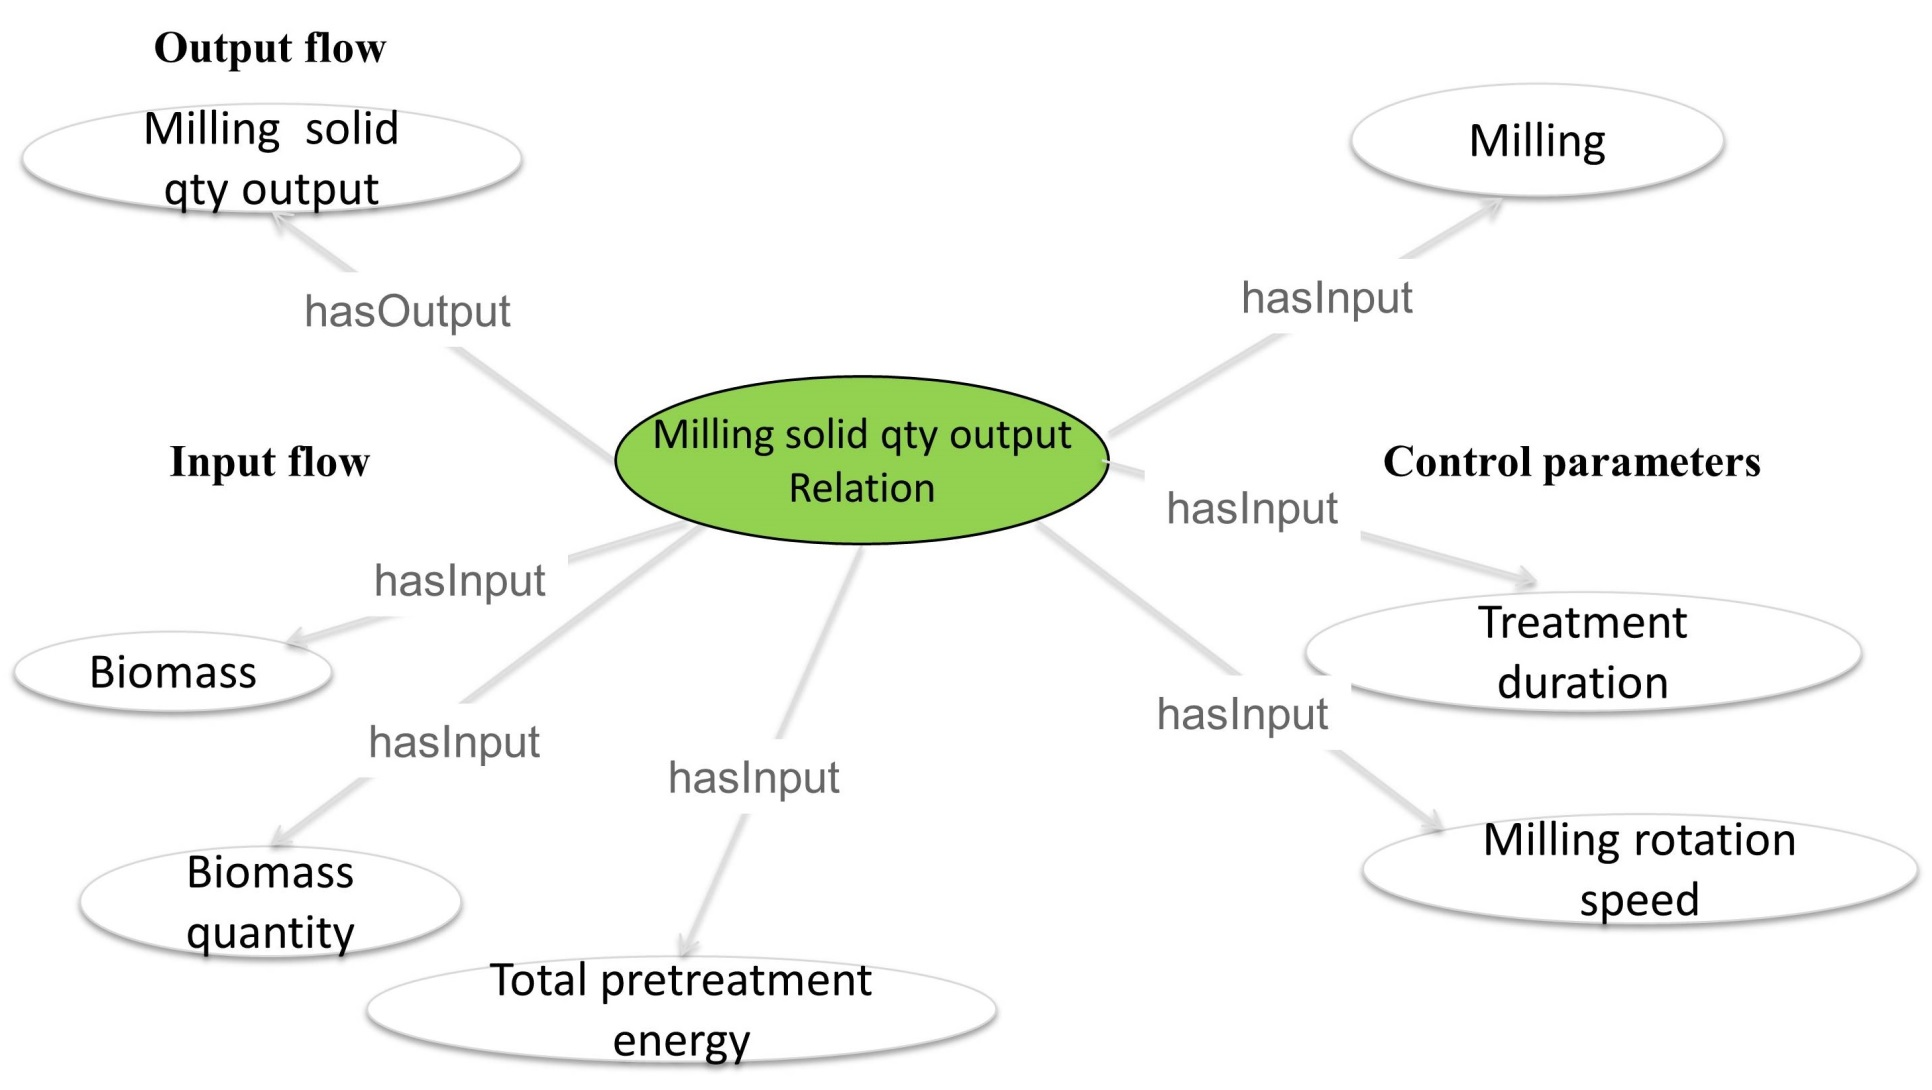
\includegraphics[width=11cm]{relation.jpg}
  \end{center}
\end{frame}

\begin{frame}
  \frametitle{An integrity constraint}
  \framesubtitle{Guideline}

  \textit{``The output quantity of a step is equal to the sum of the quantity
  of water used and the quantity of biomass present in the step.''}
\end{frame}

\begin{frame}[fragile]
  \frametitle{An integrity constraint}
  \framesubtitle{SPARQL query}

  \begin{Verbatim}[fontsize=\tiny]
SELECT ?docid ?doctitle ?tableid ?tabletitle ?rownum  ?solid_qty ?liquid_qty ?output_qty
WHERE {
?doc anno:hasForID ?docid ;
     dc:title ?doctitle ;
     anno:hasTable ?table .

?table anno:hasForID ?tableid ;
       dc:title ?tabletitle ;
       anno:hasForRow ?row .

?row anno:hasForRowNumber ?rownum ;
     anno:hasForRelation [a bioraf:milling_solid_quantity_output_relation ;
                          core:hasAccessConcept ?solid ;
                          core:hasAccessConcept ?liquid ;
                          core:hasResultConcept ?output] .

?solid a bioraf:biomass_quantity ;
       anno:hasForFS [a anno:Scalar ;
                      anno:hasForFuzzyElement /
                      anno:hasForMaxKernel ?solid_qty] .

?liquid a bioraf:water_quantity ;
        anno:hasForFS [a anno:Scalar ;
                       anno:hasForFuzzyElement /
                       anno:hasForMaxKernel ?liquid_qty] .

?output a bioraf:output_solid_constituent_quantity ;
        anno:hasForFS [a anno:Scalar ;
                       anno:hasForFuzzyElement /
                       anno:hasForMaxKernel ?output_qty] .

FILTER (xsd:float(?output_qty) != xsd:float(?solid_qty) + xsd:float(?liquid_qty))
}
  \end{Verbatim}
\end{frame}

\begin{frame}
  \frametitle{An integrity constraint}
  \framesubtitle{Graph view of the SPARQL query}

  \begin{center}
  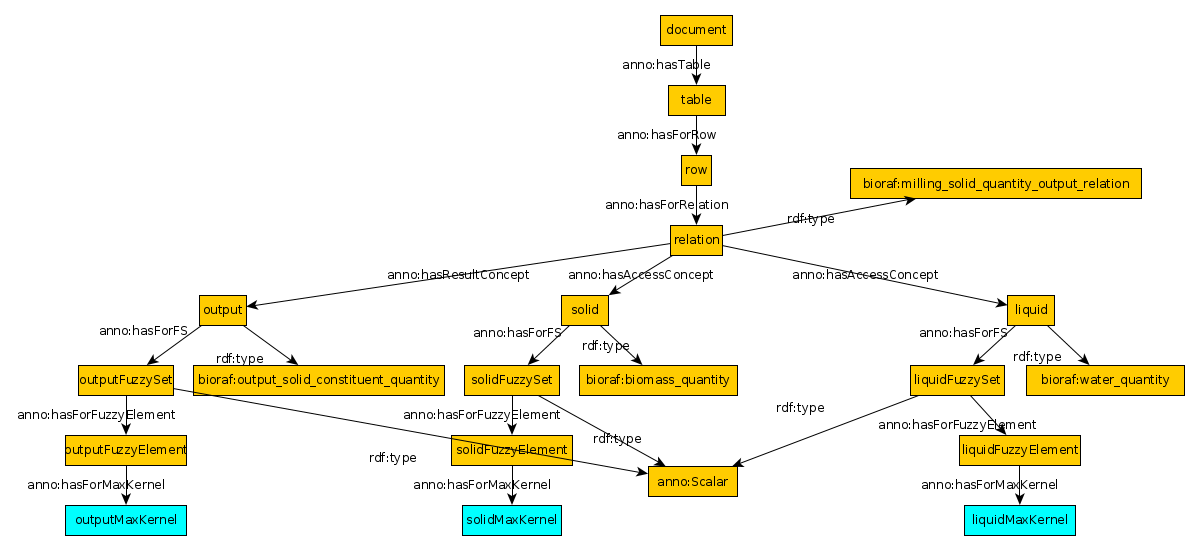
\includegraphics[width=11cm]{integrity-constraint.png}
  \end{center}
\end{frame}

\begin{frame}[fragile]
  \frametitle{An integrity constraint}
  \framesubtitle{Shape Expression}

  \begin{Verbatim}[fontsize=\tiny]
<DocumentShape> { rdf:type anno:Document, anno:hasTable @<TableShape> }
<TableShape> { anno:hasForRow @<RowShape> }
<RowShape> { anno:hasForRelation @<MillingSolidQuantityOutputRelationShape> }

<MillingSolidQuantityOutputRelationShape> {
  rdf:type bioraf:milling_solid_quantity_output_relation,
  core:hasAccessConcept @<SolidAccessConceptShape>,
  core:hasAccessConcept @<LiquidAccessConceptShape>,
  core:hasResultConcept @<OutputResultConceptShape>
}

<SolidAccessConceptShape> {
  rdf:type bioraf:biomass_quantity,
  anno:hasForFS @<FuzzySetShape>
}

<LiquidAccessConceptShape> {
  rdf:type bioraf:water_quantity,
  anno:hasForFS @<FuzzySetShape>
}

<OutputAccessConceptShape> {
  rdf:type bioraf:output_solid_constituent_quantity,
  anno:hasForFS @<FuzzySetShape>
}

<FuzzySetShape> {
  rdf:type anno:Scalar,
  anno:hasForFuzzyElement @<FuzzyElementShape>
}

<FuzzyElementShape> { anno:hasForMaxKernel xsd:string }
  \end{Verbatim}
\end{frame}

\begin{frame}[fragile]
  \frametitle{An integrity constraint}
  \framesubtitle{SHACL shapes graph (I)}

  \begin{columns}[t]
    \column{0.5\textwidth}

    \begin{Verbatim}[fontsize=\tiny]
anno:MillingSolidOutputQuantityRelationshipShape
  a sh:Shape ;
  sh:scopeClass bioraf:milling_solid_quantity_output_relation ;

  sh:filterShape [
    sh:inverseProperty [
      sh:predicate anno:hasForRelation ;
      sh:valueShape [
        sh:inverseProperty [
          sh:predicate anno:hasForRow ;
          sh:valueClass anno:Table ;
          sh:minCount 1 ;
          sh:maxCount 1 ;
        ] ;
      ] ;
      sh:minCount 1 ;
      sh:maxCount 1 ;
    ]
  ] ;

  sh:property [
    sh:predicate core:hasAccessConcept ;
    sh:qualifiedValueShape [
      sh:property [
        sh:predicate rdf:type ;
        sh:hasValue bioraf:biomass_quantity
      ]
    ] ;
    sh:qualifiedMinCount 1 ;
    sh:qualifiedMaxCount 1 ;
  ] ;
    \end{Verbatim}

    \column{0.5\textwidth}

    \begin{Verbatim}[fontsize=\tiny]





sh:property [
  sh:predicate core:hasAccessConcept ;
  sh:qualifiedValueShape [
    sh:property [
      sh:predicate rdf:type ;
      sh:hasValue bioraf:water_quantity
    ]
  ] ;
  sh:qualifiedMinCount 1 ;
  sh:qualifiedMaxCount 1 ;
] ;

sh:property [
  sh:predicate core:hasResultConcept ;
  sh:valueClass bioraf:output_solid_constituent_quantity ;
  sh:minCount 1 ;
  sh:maxCount 1 ;
] ;
    \end{Verbatim}
  \end{columns}
\end{frame}

\begin{frame}[fragile]
  \frametitle{An integrity constraint}
  \framesubtitle{SHACL shapes graph (II)}

  \begin{Verbatim}[fontsize=\tiny]
  sh:constraint [
    sh:predicate anno:width ;
    sh:sparql """
      SELECT $this ($this AS ?subject)
             (CONCAT("Output quantity must be the sum of the solid and liquid input quantities
                      (solid=", STR(?solid_qty),
                     ", liquid=", STR(?liquid_qty),
                     ", output=", STR(?output_qty), ")") as ?message)
      WHERE {
        $this core:hasAccessConcept ?solid ;
              core:hasAccessConcept ?liquid ;
              core:hasResultConcept ?output .

        ?solid a bioraf:biomass_quantity ;
               anno:hasForFS [a anno:Scalar ;
                              anno:hasForFuzzyElement /
                              anno:hasForMaxKernel ?solid_qty] .

        ?liquid a bioraf:water_quantity ;
                anno:hasForFS [a anno:Scalar ;
                               anno:hasForFuzzyElement /
                               anno:hasForMaxKernel ?liquid_qty] .

        ?output a bioraf:output_solid_constituent_quantity ;
                anno:hasForFS [a anno:Scalar ;
                               anno:hasForFuzzyElement /
                               anno:hasForMaxKernel ?output_qty] .

        FILTER (xsd:float(?output_qty) !=
                xsd:float(?solid_qty) + xsd:float(?liquid_qty))
      }
    """ ;
] .

  \end{Verbatim}
\end{frame}

\begin{frame}
  \frametitle{SHACL, ShEx and raw SPARQL pros and cons (I)}

  SHACL pros:

  \begin{itemize}
    \item Constraints are represented as RDF triples; no additional storage
      medium needed.
    \item Rich core constraints vocabulary.
    \item Possible to define arbitrary constraints using SPARQL.
    \item SHACL implementation readily available (Java language).
    \item Already being used in the industry (TopQuadrant).
  \end{itemize}

  SHACL cons:

  \begin{itemize}
    \item Constraints involving properties from different nodes require
      describing the graph structure within SPARQL queries, rendering the
      SHACL shapes redundant.
  \end{itemize}
\end{frame}

\begin{frame}
  \frametitle{SHACL, ShEx and raw SPARQL pros and cons (II)}

  ShEx pros:

  \begin{itemize}
    \item Conceptually simple, familiar model inspired in regular languages.
    \item Extensible by means of semantic actions.
  \end{itemize}

  ShEx cons:

  \begin{itemize}
    \item No feature complete implementations available at the moment.
    \item Semantic actions are not fully specified in the current draft.
    \item Requires learning a new language.
    \item Constraints over paths require defining lots of intermediate shapes
      for internal nodes in the paths.
  \end{itemize}
\end{frame}

\begin{frame}
  \frametitle{SHACL, ShEx and raw SPARQL pros and cons (III)}

  Raw SPARQL pros:

  \begin{itemize}
    \item Well known; technology and tooling readily available.
    \item Doesn't require introducing new dependencies into the \atweb stack.
    \item Complex constraints can be implemented with less code compared to
      SHACL and ShEx.
  \end{itemize}

  Raw SPARQL cons:

  \begin{itemize}
    \item Simple constraints can be more easily and briefly expressed with SHACL
      and ShEx.
    \item Harder than SHACL and ShEx, except for the cases where SPARQL code
      is needed for custom constraints.
  \end{itemize}
\end{frame}

\begin{frame}
  \begin{center}
    \Huge{Thanks!}
  \end{center}
\end{frame}

\end{document}
